\chapter{Evaluation}
\label{ch:evaluation}
\vspace{-25pt}
This chapter presents the experimental evaluation to demonstrate the advantages of employing the \sic
quality metric in a stream processing system. All experiments are performed using the \sys prototype
implementation described in Chapter~\ref{ch:system_design}.
The research questions that this chapter addresses aim at a better understanding of the characteristics
of the \sic metric and its applicability in the context of a continuously overloaded stream
processing system.
The \sic metric is designed to be operator agnostic. It can be applied to a general purpose
system supporting any type of query, providing an indication of the quality of the
computed results. This chapter considers the following research questions. Does the \sic value reflect
the correctness of the delivered results? 
What is the correlation between the error of the output and the reduction in \sic values?\\
In addition, the \sic metric is used for the implementation of semantic shedding policies.
We design a fair shedding policy and compare its performance to that of a random
shedder.
Does such a policy achieve better quality results? Is it more fair in the allocation of system
resources?\\
We were also interested in evaluating the performance of such a fair shedding policy in terms of
scalability, both when varying the number of nodes and the number of deployed queries.
What is the behaviour of the fair shedder when the amount of processing resources
changes? Does its performance scale linearly with the number of processing nodes? What happens when the
number of queries is increased on the same processing infrastructure? \\
A user may be willing to trade off the correctness of result with a reduction of costs, \eg by
deploying a larger number of queries on the same processing infrastructure. 
Is it possible to strike a balance between the achieved \sic value and the cost of paying for the
processing infrastructure? Adding an increasing number of queries to the system reduces the cost per
query.
How does this reduction in cost correlate with the reduction in \sic values? All these questions are
answered in this chapter by considering a range of sample queries using both synthetic and real-world
input data.
%\todo{fill page, fix table workload}
%\clearpage


\section{Experimental Set-up}

This section describes the experimental set-up used in this chapter. We use two testbeds: a local one and
the Emulab testbed, as described in Table~\ref{table:machines}. The local testbed consists of three
machines with 1.8~Ghz~CPUs and 4~GB of memory running Ubuntu Linux 2.6.27-17-server. They are connected
over a 1~Gbps network.
One machine is used as an oracle with a global system view, one for the input sources and query
submission and one as a processing node.
The Emulab testbed consists of a varying number of pc3000-type machines connected over a 1~Gbps LAN network. 
Each machine has a 3~Ghz CPU, 2~GB of memory and runs the FBSD410+RHL90-STD Emulab-configured Linux
image. One machine is used as an oracle, three as input sources and three for the submission of queries.
 
The workloads chosen for the experiments belong to two query classes:  
aggregate (\ie \textnormal{AVG}
%, \textnormal{MAX} 
and \textnormal{COUNT}) and complex (\ie \textnormal{TOP-5} and 
\textnormal{COV}) queries. They are summarised in Table~\ref{table:queries}. 
The queries use a diverse set of operators, namely: \textnormal{average}, 
%\textnormal{max},
\textnormal{top-k}, \textnormal{group-by}, \textnormal{filter}, \textnormal{join}, \textnormal{covariance}, 
\textnormal{time-window}, \textnormal{remote-sender}, \textnormal{remote-receiver} 
and \textnormal{output}. The first query class consists of two aggregate queries, chosen to
investigate the behaviour of the \sic metric under different operator semantics. 
The second class consists of more complex queries used to explore the properties of the \sic metric in
workloads with a broader variety of operators, beyond just the aggregate domain.
These query types are representative for a variety of data processing applications, such as sensor
networks and social media analysis.\\
%% --- TABLE TESTBED ---

%% --- TABLE TESTBED ----
\begin{table}[b!]
  %\centering
  \hspace{0.8cm}
  \renewcommand{\arraystretch}{1.5}
  \begin{tabular}{|m{3cm}|p{12cm}|} 
  \hline
  \multicolumn{2}{|c|}{\bf Local Testbed} \\ 
  
    \hline\hline
	Physical configuration
	& 
	3 machines with 1.8~Ghz CPUs and 4~GB of memory running Ubuntu Linux 2.6.27-17-server and connected
	over 1~Gbps network. \\
    \hline
	
	System layout
	&
	1 machine: oracle node; 1 machine: source data generation and query submission; 1 machine: \sys
	processing node. \\
    \hline
	
	Data sources
	&
	400~tuples/sec in 5~batches/sec of 80~tuples/batch. 
	\\
    \hline\hline
    
    \multicolumn{2}{|c|}{\bf Emulab Testbed} \\ 
    \hline\hline
	Physical layout
	&	
	pc3000-type machines connected over a 1~Gbps LAN network. Each machine has a 3~Ghz CPU, 2~GB of
	memory and runs the FBSD410+RHL90-STD Emulab-configured Linux image.
	\\
    \hline
	System layout
	&
	1 machine: 1 oracle node;
	3 machines: source data generation; 
	3 machines: query submission;
	18 machines: 18 \sys processing nodes. \\
    \hline
	
	Data sources
	& 
	150~tuples/sec in 3~batches/sec of 50~tuples/batch. \\
	
    \hline\hline 
  \end{tabular}
  \caption{Testbed configurations for experiments. }
  \label{table:machines}
\end{table}

%% --- TABLE QUERIES ---
%% --- TABLE QU1ERIES ---
\begin{table}[h!]
  \centering
  \renewcommand{\arraystretch}{1.5}
  \begin{tabular}{|m{3cm}|p{12cm}|}
    \hline
    \multicolumn{2}{|c|}{\bf Aggregate Queries} \\ 
    \hline\hline
    \textnormal{AVG}	&  Calculates the average value over 1~sec. \\ 
%     \hline
%     \textnormal{MAX}	&  Calculates the maximum value over 1~sec. \\ 
    \hline	  
    \textnormal{COUNT}	&  Counts the number of tuples with values $>=$ 50.0 over 1~sec.  \\  
    \hline\hline
    \multicolumn{2}{|c|}{\bf Complex Queries} \\ 
    \hline \hline
    \textnormal{TOP-5}	&  Shows the 5~PlanetLab nodes with the
    highest amount of available CPU and at least 100~KB of free memory over 1~sec.\\
    \hline	  
%     \textnormal{AVG-all} & Shows the avg CPU consumption over
%     PlanetLab nodes over 1~sec. \\
%     \hline	  
    \textnormal{COV} &  Shows the covariance of the CPU cycles consumption between two PlanetLab nodes.
    \\
    \hline	  
  \end{tabular}
  \caption{Query workload for experiments.}
  \label{table:queries}
\end{table}

%% --- TABLE INPUTS ---
%% --- TABLE TESTBED ----
\begin{table}[h!]
  \centering
  \renewcommand{\arraystretch}{1.5}
  \begin{tabular}{|m{3cm}|p{12cm}|} 
  \hline
  \multicolumn{2}{|c|}{\bf Synthetic source data} \\ 
  
    \hline\hline
	Gaussian
	& 
	Gaussian data distribution of mean 50. \\
    \hline
	
	Uniform
	&
	Uniform data distribution of mean 50.
	\\
    \hline
	
	Exponential
	&
	Exponential data distribution of mean 50.
	\\
	\hline
	
	Mixed
	&
	Random mix from the gaussian, uniform and exponential input sets.
	\\
    \hline\hline
    
    \multicolumn{2}{|c|}{\bf Real-world source data} \\ 
    \hline\hline
	PlanetLab
	&	
	CPU and memory measurements collected on PlanetLab in April 2010 by the CoTop project. 
	\\
    \hline    
  \end{tabular}
  \caption{Input source data for experiments.}
  \label{table:inputs}
\end{table}


The input data generated by the sources contains either real-world load measurements or a specific
synthetic workload.
The real-world data streams are log traces of CPU load and memory usage measurements from all PlanetLab
nodes~\cite{planetlab} collected in April~2010, as recorded by the CoTop
project~\cite{cotop}.
The values of the synthetic data follow either a \emph{gaussian}, \emph{uniform} or \emph{exponential}
distribution, as described in Table~\ref{table:inputs}.
Furthermore, a \emph{mixed} synthetic workload is used that combines all three distributions randomly.
These synthetic workloads provide controlled experimental input sets that allow for an easier understanding of the results. 
In all experiments, the duration of the source time window~(STW) is set to 10~seconds for all
sources. This value stays well within the variation of processing delays of all the chosen queries.
The shedding interval is set to 250~milliseconds, a value that provides a good trade-off between
throughput and management overhead.

In the experiments using more than one processing node the deployment of
queries emulates the scenario of a federated resource pool, in which the allocation of resources
is not homogeneous. Each query is partitioned into a number of subqueries, and these fragments are
deployed on the available nodes according to a Zipf distribution~\cite{zipf}. Consider, for example,
a scenario in which the number of nodes is 20, divided into 4 clusters of 5 nodes each, with a total
number of query partitions of~150. According to the Zipf law, each cluster is assigned twice as many
subqueries as the previous one. Starting with the deployment of 10 partitions onto the first cluster, the
second receives 20, the third 40 and the fourth 80. 

%% --- TABLE INPUTS ----  
% The \textnormal{AVG}, \textnormal{COUNT} and \textnormal{MAX} aggregate queries connect to one source
% with a rate of 400~tuples/sec, grouped in 5 batches of 80 tuples each.
% The \textnormal{TOP-5} query connects to 20~sources, equally split between CPU load and memory readings.
% Each source has a rate of 20~tuples/sec grouped in 5 batches of 4 each (a total of 400~tuples/sec).
% %The mean for the ten CPU sources is increased from 50 to 230 in steps of 20. 
% Th \textnormal{COV} queries connect to two sources, providing CPU readings with a rate of 200~tuples/sec,
% grouped in 5 batches od 40 tuples each (a total of 400~tuples/sec). 
% 
% The load of 400 tuples/sec was chosen empirically \ldots
%  

%--------------------------------------------------------------------------------------------------------
  

\vspace{-10pt}
\section{SCR Values and Correctness}

First, we evaluate the correlation between the \sic values of the output tuples and the correctness of
the computed results across a representative range of \emph{aggregate} and \emph{top-k} classes of
queries (see Table~\ref{table:queries}). 
The experiments use the synthetic workload as well as real load measurements collected on PlanetLab
(see Table~\ref{table:inputs}).
% Furthermore, we also include the calculation of the covariance
% metric between two time-series data of real numbers which is widely used in statistics and scientific processing to measure the correlation between two variable.
% \mnote{What are these time-series and where are they used? Probably there should be a citation.}
% 
% When using the SCR metric to provide feedback on processing quality to users,
% it is important that performance of the result of the query output is 
% \emph{strictly increasing} to the SCR values: \ie as the SCR values increase,
% the query result output is getting \emph{closer} to the perfect result 
% without shedding or it does not change. 
% \mnote{This text is from the paper. I agree on the ``stictly increasing'' argument.}
%
%\subsection*{Experimental Setup}

For this set of experiments the local testbed is used (see Table~\ref{table:machines}). A single \sys
processing node is overloaded by instantiating an increasing number of queries of one class. As we increase the number of queries, the node is forced to discard
more input tuples. The node uses a load-shedder that discards tuples randomly from each query.
The experiment is repeated for every query class and for each of the five different sets of source data. 
\vspace{-10pt}
\subsection*{Correlation Metrics}

We compare the results of a query with degraded processing (\ie with result SCR values of less
than~1) against the result of a query with perfect processing. Each query, degraded and perfect, runs
for 5~minutes and the error in the results is measured every second as a function of the achieved SCR
value. For each query class, the experiment is repeated for all the different input data sets.

%For the \textnormal{AVG}, \textnormal{COUNT} and \textnormal{MAX} aggregate 
For the \textnormal{AVG} and \textnormal{COUNT} aggregate 
queries, we use the \emph{mean absolute error} (MAE) to quantify the relative distance of the
\emph{degraded} from the \emph{perfect} result value across all
measurements for the duration of the experiment:
\vspace{-10pt}
\begin{align}
%\text{MAE} = \frac{1}{n} \mathlarger{‎‎\sum}{\left\lvert {\displaystyle \frac{\displaystyle
%\mathit{degraded} -
%\displaystyle
%\mathit{perfect}}{\displaystyle \mathit{perfect}}}} \right\rvert
\end{align}

For the \textnormal{TOP-5} query, we calculate the error using the
Kendall distance metric~\cite{kendall} that counts the differences (\ie permutations and
elements in only one list) of pairs of distinct elements between the two
lists. 
The Kendall's distance $\tau$ is defined as:
\begin{align}
\tau = \frac{C_p-D_p}{\frac{1}{2} n (n-1)}
\end{align}
where $C_p$ is the number of concordant pairs, $D_p$ is the number of discordant pairs and $n$ is the
total number of pairs. This value is normalised to lie within the [0,1] interval.

In the case of the \textnormal{COV} query, we compare the standard deviation of the real covariances
with the one under overload. The real covariance comes from perfect processing, and its value is matched
with the covariance obtained for degraded processing. Hence, we can evaluate the correlation between the
\sic values and the quality of the \textnormal{COV} query results.
% The duration of each experiment is 5~minutes each and the \textnormal{COV} query outputs a new
% \emph{sample} covariance every 1~sec. 
  
%--------------------------------------------------------------------------------------------------------
\subsection*{Experimental Results}
The following graphs show the results from the experiments running queries belonging to the
\emph{aggregate} and \emph{complex} classes. A graph is shown for each query type (\textnormal{AVG},
\textnormal{COUNT}, \textnormal{TOP-5} and \textnormal{COV}). Each graph contains the
measurements from the different runs of the experiment, one for each input data~set.

\paragraph{Aggregate queries.}
For the \textnormal{AVG} queries (see Figure~\ref{fig:agg-avg}), the graph shows a small error even
under heavy overload. This is due to the particular nature of the average operation. Since the
load-shedder discards tuples at random, the distribution of the data is not significantly affected. 
However, we observe that, as the amount of \mbox{load-shedding} diminishes and the SCR values increase,
the degraded values are closer to the perfect ones.

The \textnormal{COUNT} query (see Figure~\ref{fig:agg-count}) shows a different behaviour. The error
grows linearly with the amount of discarded data. This is an extreme case, in which the occurrence of
\mbox{load-shedding} has always a direct effect on the final results. Each tuple that is discarded, in fact,
reduces the total output value (\ie the final count) and thus increases the error.
\vspace{15pt}
% In the case of the \textnormal{MAX} query (see Figure~\ref{fig:agg-max}), we note that the result has a
% small error for the synthetic distributions. However, the error increases and shows a linear correlation in the
% case of the mixed and the PlanetLab distributions. The reasons for this difference in behaviour could be
% due to the different nature of the data sets. In the uniform, exponential and gaussian data sets, the
% data is arranged according to a regular distribution, thus a random reduction of the input data does not 
% modify the difference in absolute terms. For the PlanetLab and Mixed data sets instead, the input values
% are more scattered and have a lower regularity. \todo
% ---- AVG FIGURE -----
\begin{figure}[h!]
\centering
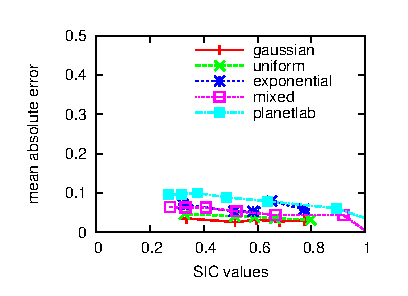
\includegraphics[width=0.55\textwidth]{img/tesi/avg1}
\caption{Correlation of SCR values with the query output quality for \emph{average} queries.}
\label{fig:agg-avg}
\end{figure} 
\clearpage

% ---- COUNT FIGURE -----
\begin{figure}
\centering
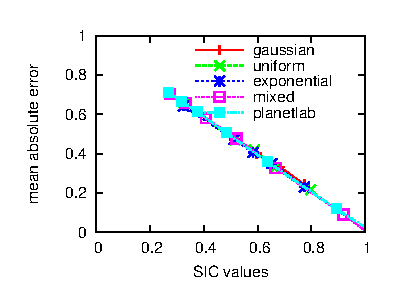
\includegraphics[width=0.55\textwidth]{img/tesi/count1}
\caption{Correlation of SCR values with the query output quality for \emph{count} queries.}
\label{fig:agg-count}
\end{figure}
% % ---- MAX FIGURE -----
% \begin{figure}
% \centering
% \label{fig:max}
% 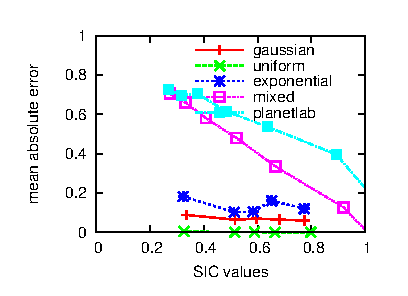
\includegraphics[width=0.6\textwidth]{img/tesi/max1}
% \caption{Correlation of SCR values with the query output performance for \emph{Max} queries.}
% \label{fig:agg-max}
% \end{figure}
%--------------------------------------------------------------------------------------------------------
\paragraph{Complex queries.}
For the \textnormal{TOP-5} query (see Figure~\ref{fig:top5}), the error expressed as the Kendall distance
decreases almost linearly with the amount of \mbox{load-shedding} performed, showing a good correlation
between the \sic metric and the correctness of results for this type of query. 
%The abnormal data point in the exponential distribution is most probably an outlier, due to some
%undetected problem with the experimental setup.

For the \textnormal{COV} query (see Figure~\ref{fig:cov}), the standard deviation of results shows a
decreasing trend as the amount of \mbox{load-shedding} diminishes and the \sic value increases. This means that
when the amount of overload is reduced, the spread in the value of the results is also reduced.
All input distributions, real and synthetic, show a low error despite the large amount of
\mbox{load-shedding}. 
% Only the exponential distribution suffers from a larger error, even with limited overload.
% This behaviour is due to the nature of the data distribution. \todo

Even for this other set of queries, the experimental results show a good correlation between the achieved
\sic values and the correctness of the results. The severity of the overload condition is, in general,
directly proportional to the error observed in the output results. This means that, although the \sic
metric is designed as a generic quality metric, it provides a good indication of the quality of the
computed results.
\begin{figure}[h!]
\centering 
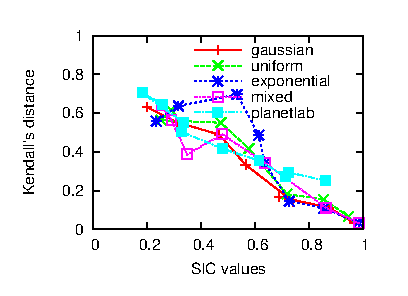
\includegraphics[width=0.55\textwidth]{img/tesi/topK-distance}
\caption{Correlation of the SCR values with the query output quality for \emph{top-5} queries.}
\label{fig:top5}
\end{figure}
\clearpage
% ---- COVARIANCE FIGURE -----
\begin{figure}[h!]
\centering
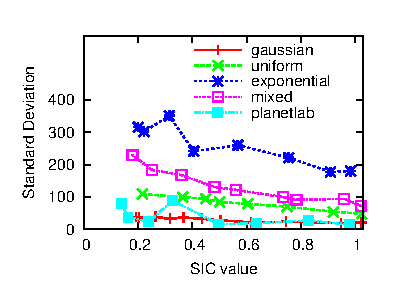
\includegraphics[width=0.55\textwidth]{img/tesi/cov}
\caption{Correlation of the SCR values with the query output quality for \emph{covariance} queries.}
\label{fig:cov}
\end{figure}% The results show that there in most cases there is a strictly increasing 
% correlation between the result SCR values and the distance/error to the perfect result: 
% the more the SCR values increase, the smaller the error. The degree of correlation 
% depends on the type of query and the source data
% distribution. When tuples are discarded randomly, tuples with values across the
% range of the initial distributions are chosen at random. The distribution of
% the values of admitted tuples are correlated with the original distribution.


\section{\mbox{Load-shedding} Policies}
\label{sec:ls-eval}

This section describes experiments that evaluate the use of the \sic quality metric for
\mbox{load-shedding}. Using the \sic metric, it is possible to implement \emph{semantic shedding
policies}~\cite{sem-ls} that discard tuples based on their information content.
% The \sic metric measures the amount of failure that occurred during the creation of a tuple and is thus
% an indication of the quality of the data.
These experiments evaluate a \emph{fair shedding} policy (see Section~\ref{sec:fair-shedding}), which is
designed to provide an equal allocation of system resources, with the goal of equalising the
quality of processing (\ie same \sic value) for all running queries under continuous overload.
We compare the fair shedding to a random shedding policy.
% The fair shedding policy is an implementation of the algorithm presented in
% Section~\ref{sec:fairness-algo}.
% The goal of this policy is to achieve fairness in the resource allocation for all queries running into
% the system.
% The policy strives to equalise the SCR values achieved by the result tuples of all queries.

\subsection*{Fairness Comparison}
This section compares the random and the fair load-shedding policies. 
The fair shedder selects the tuples to be discarded in a way that equalises the processing
degradation of all queries so that their normalised (\ie in the [0,1] interval) result SCR values are numerically
close.
The random shedder, instead, picks the tuples to be discarded at random.
Our results shows that the fair shedder always outperforms the random shedder,
achieving a higher average quality of the results (mean) and also a lower spread, measured
using a sort of dispersion metrics (IQR, Q.95-Q.05 and STD).
The experimental set-up for this set of experiments consists of 25 Emulab nodes, as described in
Table~\ref{table:machines}.
The query workload is a mix of three different queries: average, covariance and top-5, as described in
Table~\ref{table:queries}. 

Each run of the experiment compares the performance of the random and fair shedding policies, varying the
number of query partitions (\ie subqueries) for each query, while trying to maintain a similar total
number of queries. 
This means that, if the number of partitions per query increases, the total number of queries
decreases (see Table~\ref{table:partitions}). 
A larger number of subqueries distributes the load of each individual query over
a larger number of nodes, increasing the overhead due to the inter-node network communication.
The goal is to explore the effect of increasing the number of partitions for the same number of queries,
while comparing the two load-shedding policies.

Table~\ref{table:partitions} shows a breakdown of the workload characteristics for each experimental run.
The first column lists the number of subqueries that each query has been partitioned into, the second
column shows the total number of deployed queries, and the final column shows the total number of
subqueries deployed. The last row contains the data for the \emph{mixed} run, in which each query is
divided into a random number of partitions between 2 and 6.
% 
% \begin{figure}[h!]
% \centering
% 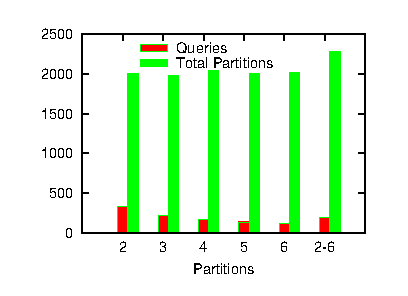
\includegraphics[width=0.6\textwidth]{img/tesi/partitions}
% \caption{Fair and random shedders comparison: IQR.}
% \label{fig:iqr}
% \end{figure}

%% --- TABLE PARTITIONS ----
\begin{table}[t]
  \centering
  \renewcommand{\arraystretch}{1.5}
  \begin{tabular}{|c|c|c|c|} 
  \hline
    %\multicolumn{4}{|c|c|c|c|}{
    \bf Partitions & \bf Queries & \bf Total Subqueries \\ 
    \hline\hline
	2 & 334 & 2004 \\
	\hline 
	3 & 220 & 1980 \\
	\hline
	4 & 170 & 2040 \\
	\hline
	5 & 134 & 2010 \\
	\hline
	6 & 112 & 2016 \\
	\hline
	2-6 & 190 & $\sim$2280 \\
    \hline
  \end{tabular}
  \caption{Workload breakdown for experiments comparing the random and fair \mbox{load-shedding}
  partitions.}
  \label{table:partitions}
\end{table}

\vspace{-10pt}
\subsection*{Statistical Measures} 
The following statistical measures are used to compare the two \mbox{load-shedding} policies. 
The first, mean, is used to evaluate the average performance of the system, while the
other three capture the dispersion of results. 
Before discussing the experimental results, we provide definitions for each of them:

\textbf{Mean:} The arithmetic mean is defined as the value obtained by summing all elements of the
sample and dividing by the total number of elements in the sample. It is used to provide an
indication of the central tendency of the data set.

\textbf{Standard deviation:} The standard deviation of a data set~\cite{std} is defined as the square
root of its variance. Variance is defined as the sum of the squared distances of each term in the
sample from the mean, divided by the total number of elements in the sample.
It shows how much variation (or dispersion) exists from the mean. A low
standard deviation indicates that the data points tend to be close to the mean, whereas a high
standard deviation indicates that the data points are spread out over a large range of values.

\textbf{Interquartile range:} The interquartile range (IQR)~\cite{upton1996understanding} is a measure of
variability based on dividing a data set into quartiles.
Quartiles divide a rank-ordered data set into four equal parts. The values that divide each part are
called the first, second and third quartiles. They are denoted by Q1, Q2, and Q3, respectively. Q1 is the
middle value in the first half of the rank-ordered data set; Q2 is the median value in the set; and Q3 is
the middle value in the second half of the rank-ordered data set. The interquartile range is equal to
Q3 minus Q1.

\textbf{Q0.95-Q0.05:} This is a measure of variability used in a similar
way to the interquartile range.
The ordered data is divided into 100 equal parts, called percentiles. Q0.95-Q0.05 captures the
spread of the middle 90\% of the ordered data values. It shows the spread
of the majority of the data values and captures a larger set of values than the IQR.

% \textbf{Median:} The median~\cite{median} is described as the numerical value separating the higher half
% of a sample, a population, or a probability distribution, from the lower half. The median of a finite list of numbers
% can be found by arranging all the observations from lowest value to highest value and picking the middle
% one. If there is an even number of observations, then there is no single middle value; the median is then
% usually defined to be the mean of the two middle values.


\subsubsection*{Experimental Results} 
\vspace{-10pt}
The first graph, in Figure~\ref{fig:mean} shows the comparison
between the random and the fair shedding policies in terms of average quality of the delivered results.
In all the experiments, the fair shedder outperforms the random one, achieving on average results
with a higher \sic value than the random shedder. \\
The last three graphs in Figures~\ref{fig:iqr},~\ref{fig:std}~and~\ref{fig:qq} show the comparison
between the random and the fair shedding policies in terms of variability. For all the dispersion
measures used, the fair shedder achieves a lower value compared to the random shedder. This means that
the fair shedder chooses a better set of tuples to be discarded, leading to a higher mean \sic value
and a lower dispersion~of~\sic~values. 
All experiments show the impact of breaking the queries into more partitions for all the analysed
measures. This is due to the higher cost of inter-node communication. A larger number of subqueries
provides a better load distribution among all the processing nodes but it also increases the total load
imposed on the system. The \emph{mean} \sic value is higher in the case of two partitions and decreases
as the number of partitions increases. The \emph{dispersion} metrics, instead, have lower values for two
partitions. Their value increases when increasing the number of subqueries.
\begin{figure}[h!]
\centering
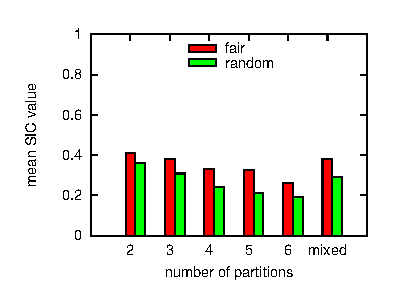
\includegraphics[width=0.55\textwidth]{img/tesi/mean}
\caption{Comparison of fair and random load shedders (MEAN).}
\label{fig:mean}
\end{figure}
\clearpage
\begin{figure}[h!]
\centering

\includegraphics[width=0.55\textwidth]{img/tesi/iqr}
\caption{Comparison of fair and random load shedders (IQR).}
\label{fig:iqr}
\end{figure}

\begin{figure}[h!]
\centering

\includegraphics[width=0.55\textwidth]{img/tesi/std}
\caption{Comparison of fair and random load shedders (Standard Deviation). }
\label{fig:std}
\end{figure}
\begin{figure}[h!]
\centering

\includegraphics[width=0.55\textwidth]{img/tesi/maxmin}
\caption{Comparison of fair and random load shedders (Q0.5-Q0.95).}
\label{fig:qq}
\end{figure}

%\clearpage

%\clearpage

%%%%%%%%%%%%%%%%%%%%%%%%%%%%%%%%%%%%%%%%%%%%%%%%%%%%%%%%%%%%%%%%%%%%%%%%%%%%%%%%%%%%%%%%%%%%%%%%%%%%%%%%%
\subsection*{Scalability of Fair Load Shedder }

The following set of experiments evaluate the scalability of the \emph{fair load shedder} in
terms of the number of nodes and queries. The aim is to observe the variation of the result \sic values
if the amount of processing resources changes. In the first set of experiments, the amount of load
remains constant, while increasing the processing resources.
Adding more nodes leads to an increase in the result \sic values because the amount of required
\mbox{load-shedding} is reduced. In the second set of experiments, the variation is in terms of
processing load, while maintaining a constant amount of processing resources. In this case, increasing
the number of deployed queries leads to a reduction of \sic values. 
% Both sets of experiments show a proportional variation of quality-of-serv ice, showing efficient
% scalability properties for the fair shedder.
Both sets of experiments are deployed on the Emulab testbed, as described in Table~\ref{table:machines}.
The processing nodes are loaded with an evenly mixed workload of
COV, AVG and TOP-5 queries, as described in Table~\ref{table:queries}.
%--------------------------------------------------------------------------------------------------------
\vspace{-10pt}
\subsubsection*{Increasing the Number of Nodes}

This set of experiments measures the scalability of the fair shedding policy in terms of
number of nodes, when varying the amount of processing
resources. Increasing the number of nodes with a fixed number of queries,
progressively reduces the overload on each processing node. The fair shedder should achieve a
proportionally better processing quality in terms of the mean \sic value. Ideally, reducing the number of
nodes by 50\% should result in the same reduction in the \sic values of the~computed~results.

Figure~\ref{fig:scalability:nodes} shows the results obtained after running the experiment on a number of
nodes varying from 9 to 24. Increasing the number of processing nodes reduces the average load
on each node and thus the need for \mbox{load-shedding}. The higher amount of available processing
resources leads to an increase in average \sic values of the output tuples. 
All dispersion measures show a reduction, which means that a better result is also achieved in terms
of the variability of the output \sic values. The value of the dispersion measures grow together with
the value of the mean. 
\begin{figure}[h!]
\centering
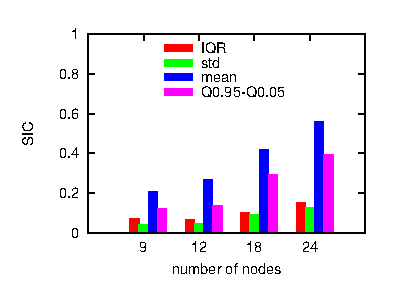
\includegraphics[width=0.55\textwidth]{img/tesi/nodes2}
\caption{Fairness for an increasing number of nodes.}
\label{fig:scalability:nodes}
\end{figure}
If the value of the mean doubles, the value of the dispersion metrics
tends to double as well because the variability range is larger. With a mean of 0.2, we can expect the
\sic values to be distributed in the interval [0,0.4], while with a mean of 0.4, we can expect the range
to be [0,0.8]. Since the range is doubled, the dispersion measures should also be doubled. What should
remain constant is the ratio between the dispersion measure and the mean, as observed this stable
ratio between the standard deviation and the mean is referred to as \emph{coefficient of
variation}~\cite{cvar}.
\vspace{-10pt}
%------------------------------------------------------------------------------------------------
\subsubsection*{Increasing the Number of Queries}

This set of experiments observes the processing quality in terms of the \sic value when varying the
number of queries (\ie increasing the load), while maintaining a constant amount of processing resources. 
The total number of nodes used in these experiments is 25 (see Table~\ref{table:machines}).
The nodes host an increasing number of queries, with an evenly mixed workload of
COV, AVG-all and TOP-5 queries (see Table~\ref{table:queries}).

Figure~\ref{fig:scalability:queries} shows the degradation in \sic values when deploying a
number of queries that varies from 180 to 1200. The results indicate that the value of all queries is
reduced proportionally to the number of queries. From the graph, it is possible to observe that the performance
of the system is not strictly linear. The slope of the descending mean \sic values changes sign, meaning
that initially the percentile reduction in the \sic value is lower than the relative increase in
the number of queries. At a certain point, this changes and the system behaviour becomes sublinear.
The next section shows how it is possible to exploit this behaviour to expose a trade-off between the
quality of results in terms of \sic values and the resource cost per query.
\begin{figure}[h!]
\centering

\includegraphics[width=0.7\textwidth]{img/tesi/queries_large}
\caption{Fairness for an increasing number of queries.}
\label{fig:scalability:queries}
\end{figure}
\clearpage
% To better analyse the 
% Figure~\ref{fig:scalability:risk} shows the \emph{signal-to-noise} ratio, defined as the ratio between
% the mean \sic value and the standard deviation of the sample for all experimental runs. 
% The results show that the system performance is fairly stable, meaning that there is graceful degradation
% of the quality-of-service when increasing the processing load.
% % 
% \mnote{106: What else: try to be more verbose here as this is the main result.
% That using the SCR metric the fair shedder is able to use source data
% across queries more efficiently than the random. That similar result
% hold for different partitions. That the mixed is the most important result.}



% 
% \begin{figure}[t]
% \centering
% 
\includegraphics[width=0.6\textwidth]{img/tesi/risk}
% \caption{Stability of performance in terms of Mean/STD for increasing number of queries experiment.}
% \label{fig:scalability:risk}
% \end{figure}
%  
%\clearpage
%--------------------------------------------------------------------------------------------------------



\section{Trade-off between Quality of Processing and Resource Cost}
\label{sec:cost}
When the user is willing to accept approximate results, it is possible to use the \sic metric to expose
a trade-off between the quality of processing and resource cost. 
If we maintain a stable amount of processing resources, increasing the number of deployed queries
leads to a reduction of the resource cost per query. 
When the percentage of cost reduction is greater than the reduction in processing quality (\ie SIC
values) there is a cost advantage by adding more queries. 

The difference in cost, $\Delta(cost)$, is calculated as:
\begin{align}
	\Delta(cost) = \frac{C_{base}-C_x}{C_{base}}
\end{align}
where $C_{base}$ is the base resource cost for the initial deployment and $C_x$ is the resource cost of
deploying $x$ queries.

The difference in quality of processing, $\Delta(QoP)$, is calculated as:
\begin{align}
	\Delta(QoP) = \frac{QoP_{base}-QoP_x}{QoP_{base}}
\end{align}

where $QoP_{base}$ is the quality of processing value for the starting deployment and $QoP_x$ is the
quality of processing achieved after deploying $x$ queries.

The deployment of new queries is considered to be advantageous when:
\begin{align}
	\Delta(QoP)>\Delta(Cost)
\end{align}
\begin{figure} 
\centering 
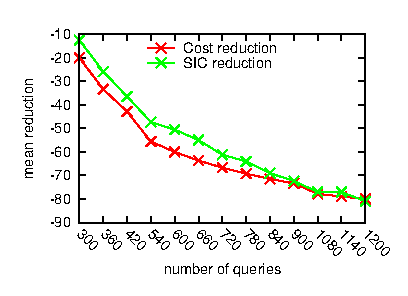
\includegraphics[width=0.6\textwidth]{img/tesi/cost2}  
\caption{Trade-off between the reduction of resource cost per query and the reduction in quality of
processing, as expressed by mean SIC values.}
\label{fig:tradeoff-mean}
\end{figure}
The difference between the reduction in cost and quality of processing is inversely proportional to the
number of queries. The more queries are added, the lower the cost advantage, until a point is reached,
at which increasing the number of queries is no longer beneficial.
% A user can keep adding new queries until this point is reached, until the difference goes under a certain
% threshold, or until a minimum SIC values is reached.
A user may add more queries until this point is reached or the difference is below a given threshold or
minimal \sic value.

\subsection*{Experimental Results}

For the trade-off evaluation, the data from Figure~\ref{fig:scalability:queries} is used. The cost of the
infrastructure remains fixed so the resource cost per query can be calculated as the inverse of the
number of queries: $1/N_{queries}$.

Figure~\ref{fig:tradeoff-mean} shows the mean \sic value as the quality of processing metric. The base
case has 180 queries and, at each step, 60 more queries are deployed. The graph shows how, with 300
queries, there is almost an 8\% difference between the reduction in quality of processing and the
resource cost reduction.
This difference grows smaller as more queries are deployed until a ``tipping point'' is reached with
approximately 900 queries. From this point onwards, adding more queries does not result in further
benefit.
% Figure~\ref{fig:tradeoff-q95} shows the same trend but uses the Q.95-Q.05 metric as the
% quality-of-service indicator.

%%\mnote{what else?}


% \begin{figure}[h!]
% \centering
% 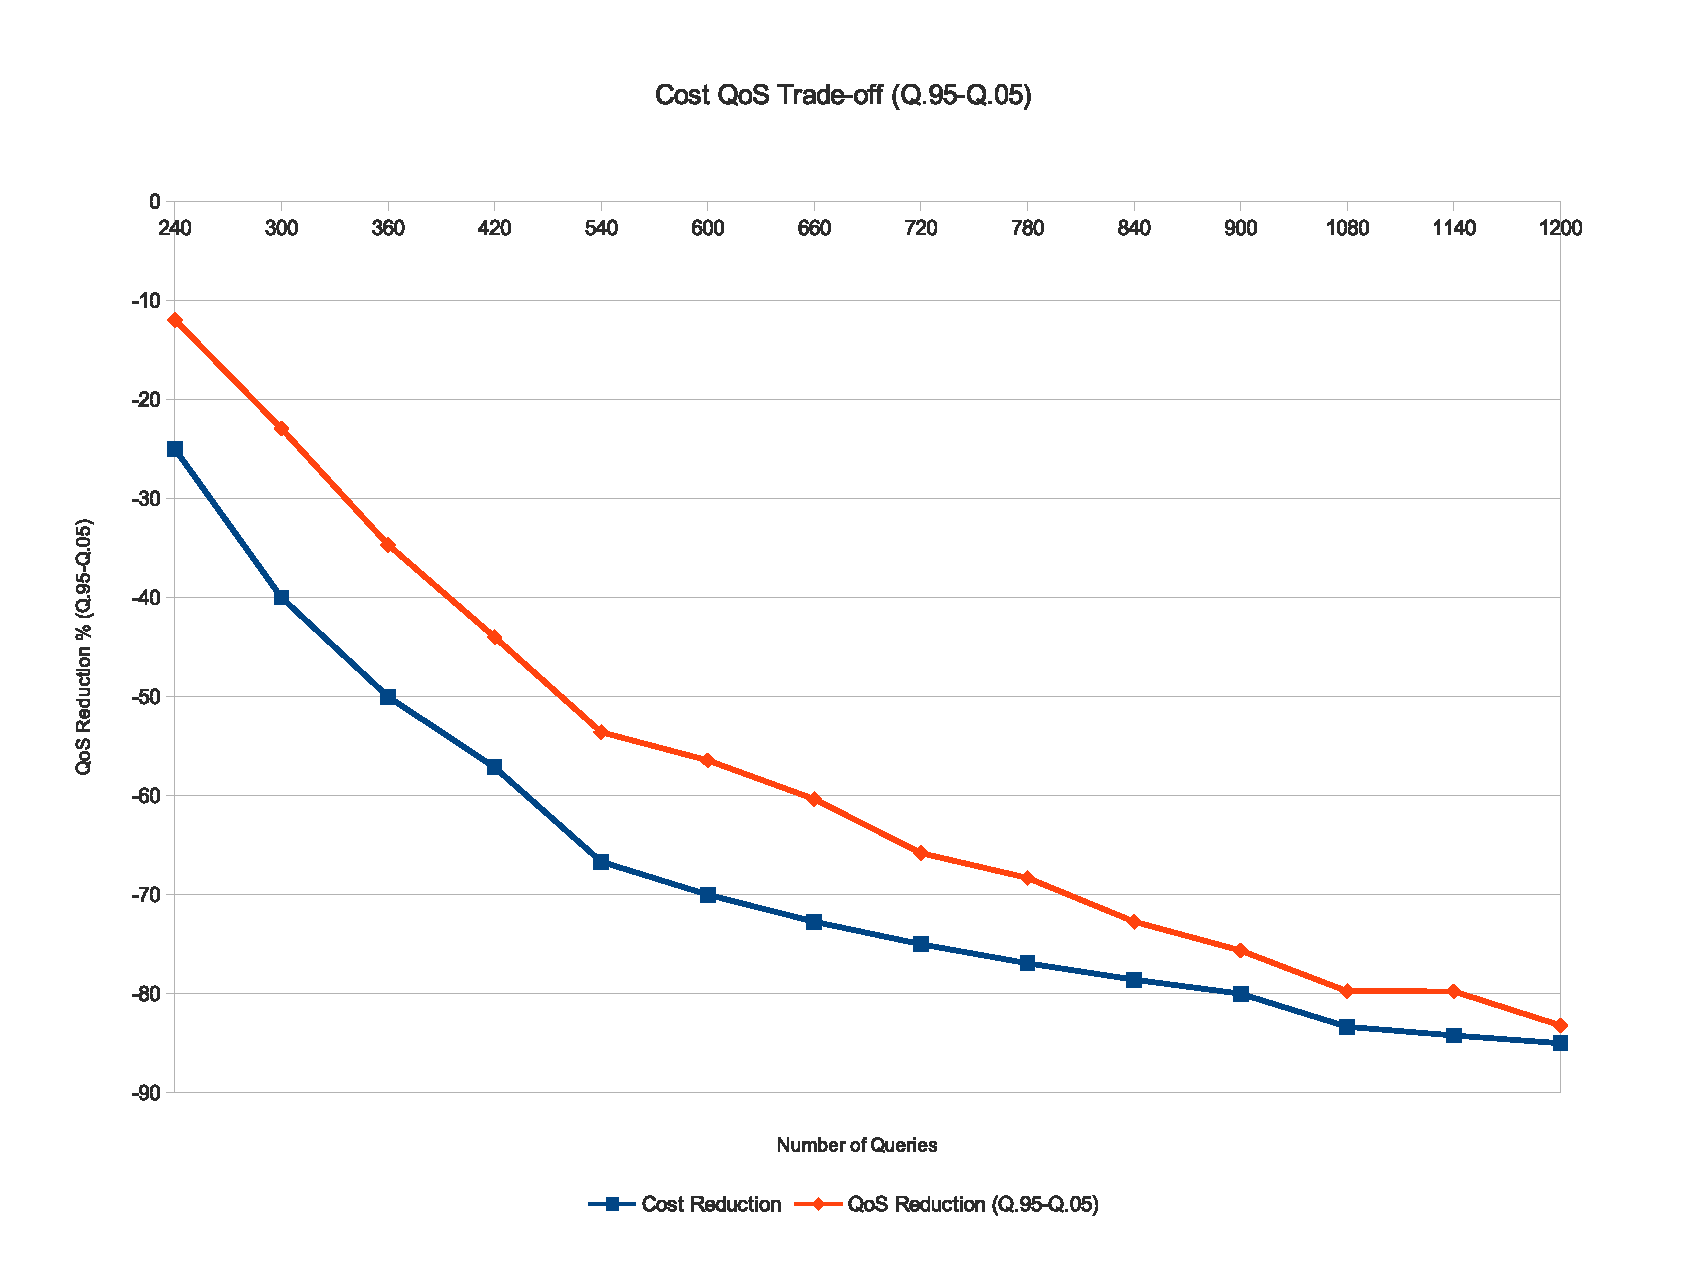
\includegraphics[width=0.6\textwidth]{img/tesi/tradeoff-q95} 
% \caption{Trade-off between the reduction of cost per query and redution in Qos expressed as Q.95-Q.05 SIC
% values.}
% \label{fig:tradeoff-q95}
% \end{figure}

%\clearpage
 

%\section{Source Time Window}
\label{sec:eval_stw}

The purpose of this set of experiments is to evaluate if the Source Time Window (STW), introduced in
Section~\ref{sec:stw} is a good approximation of the theoretical concept of Source Information Tuple
Set, introduced in Section~\ref{sec:assumptions}. In a real system it is impossible to know exactly what
tuples will contribute to the creation of a result, thus there is the need for an approximation. 
The idea is to compute \sic values over a large enough time-window that exceeds of at least an order of
magnitude the end-to-end latency of the queries. If the chose STW is too short in fact, in a normally
loaded system, it would result in a \sic value heavily fluctuating around 1. 

We evaluate the STW approximation as we increase the processing and network end-to-end latency.
To this end, we gradually grow the number of query fragments from one
to six---thus increasing the processing delay---and we deploy each fragment in a separate Emulab 
node---thus increasing the network latency---while we keep the time-window
fixed to 10~seconds. Overall, we perform six
experiments (\ie one for each number of query fragments) and for each we deploy
10 queries from each type of the complex workload mix. In all cases, \sys performs
perfect processing and the average result SCR is shown in Table~\ref{table:time-window}.
Results show a very low fluctuation of values, well within the expected range, thus meaning that the STW
approximation implemented in the \sys system correctly captures perfect processing in all cases.
\begin{table}[h]
  \centering
  \begin{tabular}{c|c||c|c}
    \hline
        fragments & SCR$\pm$std & fragments & SCR$\pm$std \\ \hline
	1 & 1.032$\pm$0.008 & 2 & 1.036$\pm$0.011 \\ \hline
	3 & 1.020$\pm$0.066 & 4 & 1.018$\pm$0.069 \\ \hline
	5 & 1.036$\pm$0.034 & 6 & 1.009$\pm$0.063 \\ \hline
  \end{tabular}
  \caption{Time-window approximation for various fragments.}
  \label{table:time-window}
\end{table}


\section{Summary}

This chapter presented the experiments performed to evaluate the advantages of employing the \sic quality
metric in a stream processing system. All experiments were carried out using the \sys prototype
system described in Chapter~\ref{ch:system_design}.  
The first set of experiments looked at the correlation between \sic values and the correctness of
results.
Even though the \sic quality metric was not designed as a direct measure of the accuracy of results,
our experiments showed that, for many classes of queries, there is a good correlation, confirming that a
high value of the \sic metric indicates a high confidence in the correctness of results.
The second set of experiments focused on the evaluation of the fair shedding policy, designed to
exploit the \sic metadata to allocate resources among queries evenly and compares its performance with
that of a random shedder. Our results showed that employing the fair shedding policy leads to a more even
distribution of \sic values for the delivered output tuples.
Finally, a set of experiments was devised to investigate the correlation between resource cost and
the processing quality of the results. 
They showed that it is possible to strike a balance between the achieved \sic values
of the results and a reduced resource cost for the processing infrastructure.


